\subsection{Surface Photometry for J1331 with MGE}

[TO DO]

\paragraph{[TO DO: Stuff to mention]}
\begin{itemize}
\item fit sof MGE to J1331s surface brightness within $\sim$ 2 half-light radii, and to an Iraf Ellipse model for J1331's outer regions, make it possible to easily deconvolve the hst images with its PSF.
\item the deporjecten if the galaxy under the assumption of oblate axusymmetry and an estimated inclination of $\sim70^\circ$ can be performed analytically.
\end{itemize}

%============================================================================

\begin{figure}
\begin{minipage}[c]{\linewidth}
\centering
\includegraphics[width=0.8\textwidth]{fig/1331F814Wsci_MGE_M.ps}
\caption{??? MGE as used in the dynamical modelling ??? [TO DO: nice caption]}
\label{fig:???}
\end{minipage}
\begin{minipage}[c]{\linewidth}
\centering
\includegraphics[width=0.8\textwidth]{fig/1331F814W_MGE_disk_L.ps}
\caption{??? [TO DO: caption]}
\label{fig:???}
\end{minipage}
\end{figure}

%============================================================================

\begin{table*}
\centering
\begin{minipage}[t]{40mm}
\caption{PSF F814W MGE ??????}
\begin{tabular}{ccc}
\hline
$k$ & $G_k$ & $\sigma_k$ [arcsec] \\\hline
1 & 0.184 & 0.038\\
2 & 0.485 & 0.085\\
3 & 0.222 & 0.169\\
4 & 0.109 & 0.487\\\hline
\end{tabular}
\label{tab:PSFMGEF814W}
\end{minipage}
\hspace{10mm}
\begin{minipage}[t]{100mm}
\caption{F814W MGE???}
\begin{tabular}{cccccc}
\hline
 & total luminosity  & surface density & \multicolumn{2}{c}{Gaussian dispersion} & axis ratio\\
$k$  & $L_k$ [counts] & $I_{0,k}$ [$L_\odot$/pc$^2$] & $\sigma_k$ [arcsec] & $\sigma_k$ [kpc] & $q'_k$\\\hline
1  &     9425.96 &      20768.  &  0.051   & 0.103  & 1.00\\
2  &    13173.0 &        3161.2 &  0.178   & 0.358  & 0.76\\
3  &    40235.0 &        1588.2 &  0.503   & 1.008  & 0.58\\
4  &    67755.2 &         502.25&  1.180   & 2.368  & 0.56\\
5  &    203677. &         136.51&  3.891   & 7.805  & 0.57\\\hline
\end{tabular}
\label{tab:MGEF814W}
\end{minipage}
\end{table*}

%============================================================================

\begin{table}
\centering
\begin{minipage}{140mm}
\caption{Galaxy Parameters of J1331}
\begin{tabular}{lllrl}
\hline
redshift                  & $z_d$ & 0.113 & \citep{SWELLSIII}\\
angular diameter distance & $D_d$ [Mpc] & 414 & \\
scaling                   & 1 kpc / 1 arcsec & 2.006 & \\
position angle            & $\phi$ [degrees] & wrt what???\\
average axis ratio & $q'$ & 0.598\\
average ellipticity & $\epsilon = 1 - q'$ & 0.402 & \\
apparent F814W magnitude & $m_\text{F814W}$ [mag] & 15.77 & \\
total F814W luminosity & $L_\text{tot,F814W}$ [$10^{10} L_\odot$] & 5.6 & \\
effective half-light radius & $R_\text{eff}$ [arcsec] & 2.6 & \\
& $R_\text{eff}$ [pc]& 5.2 & \\
\hline
\end{tabular}
\end{minipage}
\end{table}
